%%=============================================================================
%% Hoofdstuk 6: Resultaten en Discussie
%%=============================================================================

\chapter{\IfLanguageName{dutch}{Resultaten en Discussie}{Results and Discussion}}
\label{ch:resultaten_discussie}

In dit hoofdstuk worden de bevindingen uit de realisatiefase en de diagnostische analyse thematisch geëvalueerd. De focus ligt op het verklaren van de discrepantie tussen de succesvolle werking van de fysieke robot en de hardnekkige integratiefouten binnen de simulatieomgeving.

\section{Evaluatie van het Probleem- en Analysedomein}
\label{sec:evaluatie_probleem_analyse}

De centrale bevinding van dit onderzoek is dat de \textit{sim-to-real gap} in dit project niet werd veroorzaakt door fysische onnauwkeurigheden (zoals frictie of massa), maar door een fundamentele softwarematige mismatch tussen NVIDIA Isaac Sim en de ROS 2-middleware.

\subsection{De Software-to-Software Gap in de Praktijk}
Zoals beschreven in de literatuur door \textcite{Hoefer2021}, vormt de technische integratie vaak een grotere barrière dan de visuele gelijkenis. Dit werd bevestigd door het feit dat de fysieke robot, ondanks de complexiteit van de gedistribueerde rekenkracht tussen de Raspberry Pi 5 en de NVIDIA Jetson Nano, een stabiele SLAM-oplossing bood. In de echte wereld fungeerden de coördinatenstelsels (REP-103) en de temporele synchronisatie via \texttt{chronyc} naar behoren.

In de simulatieomgeving trad echter het \textit{rubberbanding}-effect op. De analyse van de verzamelde data wijst uit dat dit een direct gevolg is van de \textit{software-to-software gap}:
\begin{itemize}
    \item \textbf{Coördinaten-inconsistentie:} Ondanks de wiskundige inversies in de Action Graph (zie \ref{subsubsec:wiskundige_correcties}) en de pogingen met \textit{shadow links} in ROS, bleef er een conflict bestaan tussen de linkshandige oriëntatie van de USD-omgeving en de rechtshandige conventie van ROS 2. De data-integriteit werd aangetast op het moment dat de \texttt{isaac\_ros\_bridge} de transformaties trachtte te mappen.
    \item \textbf{Temporele Drift:} De \texttt{Isaac Read Simulation Time}-node publiceerde tijdstempels die niet consistent gesynchroniseerd waren met de systeemklok van de ROS 2 Jazzy-omgeving op de Raspberry Pi. Dit bevestigt de theorie van \textcite{Peng2020} dat zelfs minieme afwijkingen in tijdstempels leiden tot instabiliteit in de $TF$-tree, waardoor de robot in de middleware herhaaldelijk naar een eerdere logische positie ``teleporteert''.
\end{itemize}

\begin{figure}[h]
    \centering
    \begin{subfigure}{0.48\textwidth}
        \centering
        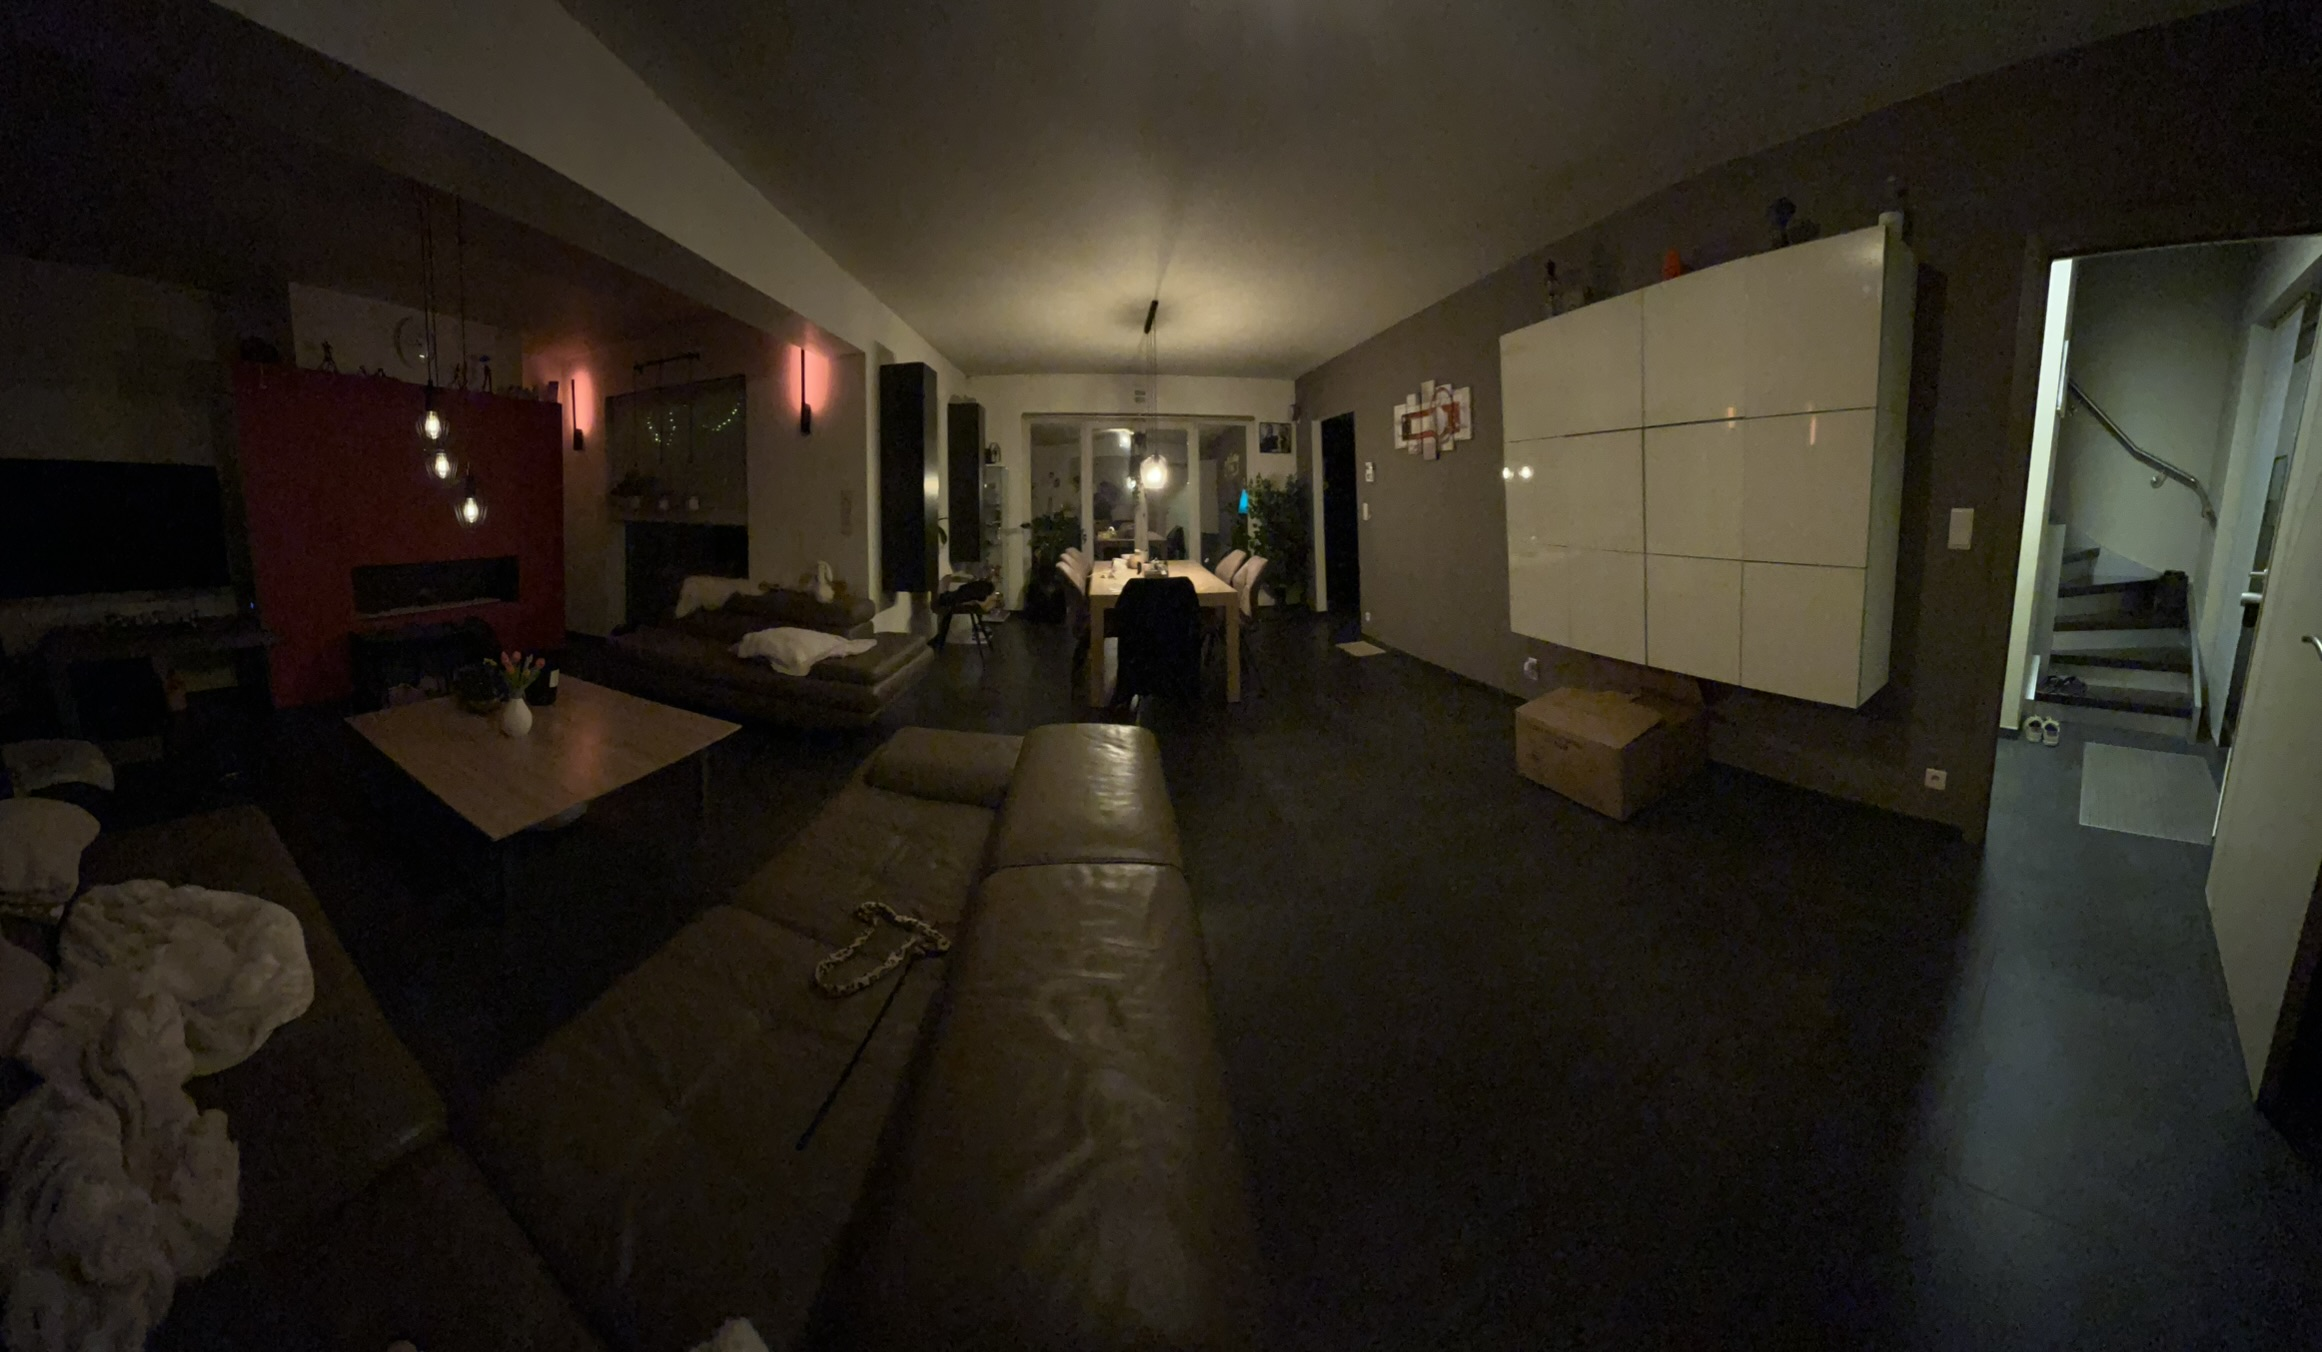
\includegraphics[width=\textwidth]{afbeeldingen/Slam/IMG_6769.JPEG}
        \caption{foto van gescande warenhuis.}
        \label{fig:WarehouseImage}
    \end{subfigure}
    \hfill
    \begin{subfigure}{0.48\textwidth}
        \centering
        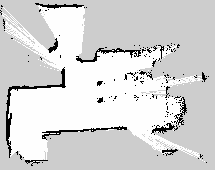
\includegraphics[width=\textwidth]{afbeeldingen/Slam/living1.png}
        \caption{Slam map resultaat van warenhuis.}
        \label{fig:WarehouseScan}
    \end{subfigure}
    \caption{Slam resultaten van fysieke robot}
    \label{fig:IRLSlamResults}
\end{figure}
\begin{figure}[h]
    \centering
    \begin{subfigure}{0.48\textwidth}
        \centering
        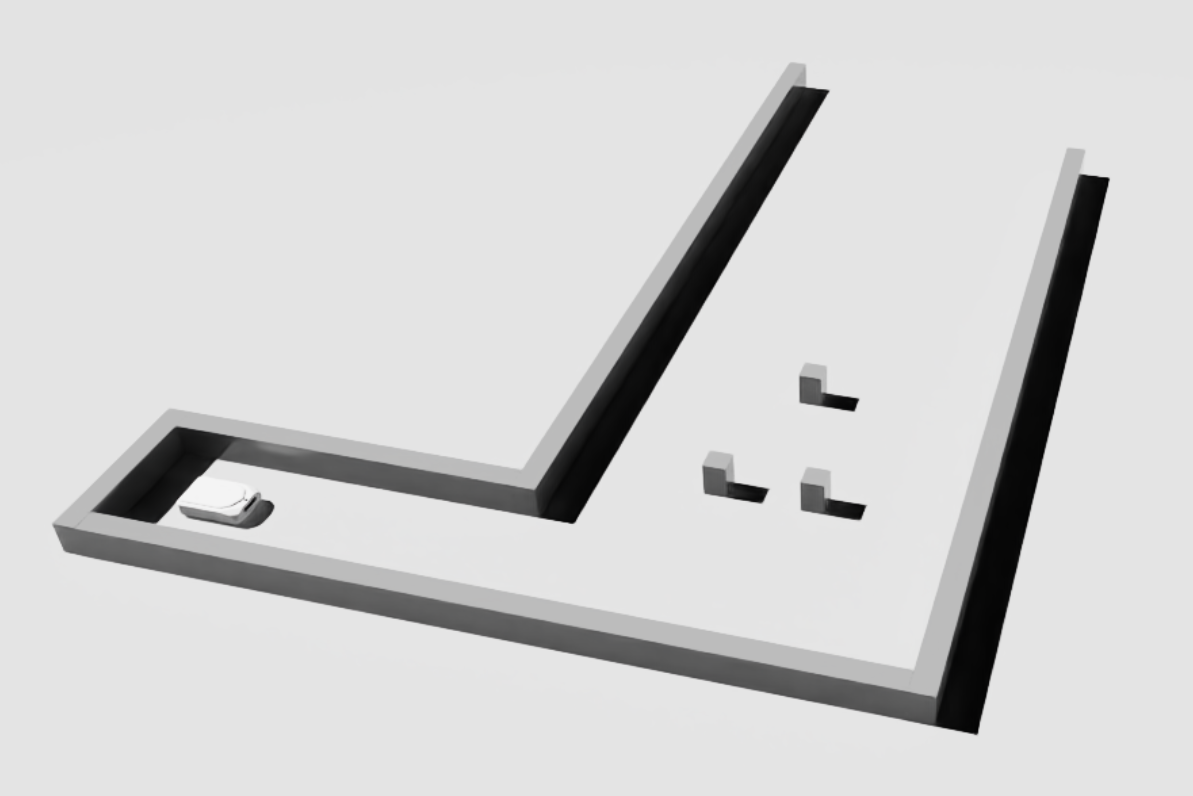
\includegraphics[width=\textwidth]{afbeeldingen/Slam/Screenshot 2026-04-21 182108.png}
        \caption{foto van virtueel warenhuis.}
        \label{fig:simWarehouseImage}
    \end{subfigure}
    \hfill
    \begin{subfigure}{0.48\textwidth}
        \centering
        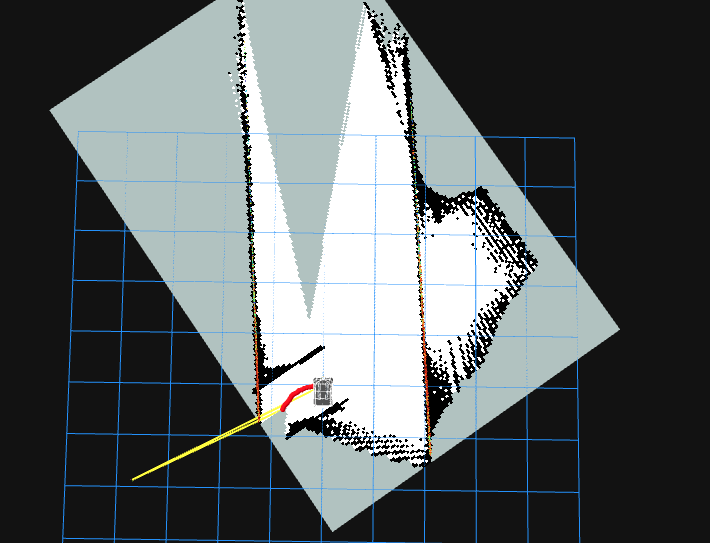
\includegraphics[width=\textwidth]{afbeeldingen/Slam/Screenshot 2026-04-22 210616.png}
        \caption{Slam map resultaat van virtueel warenhuis.}
        \label{fig:simWarehouseScan}
    \end{subfigure}
    \caption{Slam resultaten van virtuele robot}
    \label{fig:SimSlamResults}
\end{figure}

\subsection{Analyse van de Middleware-beperkingen}
Een kritieke factor in het falen van de simulatie-integratie was de verplichte overstap naar \texttt{FastDDS} voor de Windows-host van Isaac Sim. Waar de fysieke robot profiteerde van de stabiliteit van \texttt{CycloneDDS}, introduceerde de noodzakelijke configuratie voor Windows een extra laag van complexiteit en latency. De data-analyse toont aan dat pakketverlies en jitter in de odometrie-topics toenamen wanneer de simulatie-complexiteit steeg, wat de \textit{Quality of Service} (QoS) instellingen onder druk zette \autocite{Robotics2026}.

\subsection{Conclusie van de Diagnostiek}
De resultaten tonen aan dat de ``digitale tweeling'' op visueel en mechanisch vlak (via de Onshape-export) accuraat was, maar dat de communicatielaag tussen de gesloten Windows-architectuur van NVIDIA Omniverse en de open-source ROS 2-stack op Linux de zwakste schakel vormde. Het succes van de fysieke robot bewijst dat de Nav2-configuratie en de hardware-interface correct waren, wat de oorzaak van de problemen onomstotelijk in de simulatielaag positioneert. Dit benadrukt dat voor complexe \textit{under-vehicle} AMR's de standaard \textit{out-of-the-box} integraties van simulatie-bridges anno 2026 nog significante tekortkomingen vertonen bij cross-platform implementaties.

\section{Voorstel Oplossingsdomein en Aanbevelingen}
\label{sec:oplossingsdomein}

Hoewel de volledige integratie tussen de virtuele AMR en de Nav2-stack op de Raspberry Pi niet tot een productierijp resultaat leidde, biedt de diagnostische analyse voldoende inzicht om een gericht verbeterplan te formuleren. De volgende aanbevelingen dienen als leidraad voor toekomstig onderzoek en het verkleinen van de \textit{sim-to-real gap} binnen deze specifieke technologische stack.

\subsection{Architecturale aanpassingen van de Hardware en Middleware}
Een van de meest kritieke knelpunten was de noodzakelijke peer-to-peer verbinding tussen drie gescheiden rekeneenheden (Windows-host, Raspberry Pi, Jetson Nano). 
\begin{itemize}
    \item \textbf{Consolidatie van Rekenkracht:} De ``End of Life'' (EOL) status van de Jetson Nano dwong tot het gebruik van verouderde drivers en complexe netwerk-synchronisaties via \texttt{chronyc}. Een migratie naar een krachtigere, uniforme compute-unit zoals de \textbf{NVIDIA Jetson Orin-serie} wordt sterk aanbevolen. Dit zou de noodzaak voor de Raspberry Pi en de bijbehorende netwerk-latency elimineren, waardoor de volledige ROS 2-stack en de ZED SDK native op één systeem kunnen draaien onder Ubuntu 22.04 of 24.04.
    \item \textbf{Harmonisatie van ROS-distributies:} De mismatch tussen ROS 2 Humble (Isaac Sim) en ROS 2 Jazzy (Raspberry Pi) introduceerde onzekerheden in de bericht-serialisatie. Het gebruik van een identieke versie (bij voorkeur de \textit{Long Term Support} Humble-versie) op alle systemen is essentieel om protocol-inconsistenties te minimaliseren.
\end{itemize}

\subsection{Optimalisatie van de Simulatie-omgeving}
De Windows-omgeving van Isaac Sim bleek de grootste beperking voor een stabiele communicatielaag.
\begin{itemize}
    \item \textbf{Migratie naar Linux-gebaseerde Simulatie:} De Windows-versie van de \texttt{isaac\_ros\_bridge} ondersteunt momenteel geen \texttt{CycloneDDS}. Door Isaac Sim te draaien op een \textbf{Ubuntu-gebaseerde Workstation} kan \texttt{CycloneDDS} uniform over het hele netwerk worden ingezet. Dit elimineert de noodzaak voor de huidige FastDDS-omweg en verbetert de betrouwbaarheid van de transformatieboom-pakketten.
    \item \textbf{Upgrade naar Isaac Sim 6.0.0 (Isaac Lab):} Tijdens dit onderzoek is Isaac Sim 6.0.0 (onderdeel van het vernieuwde Isaac Lab) gelanceerd. Deze versie bevat verbeterde implementaties van de \textit{ROS 2 Bridge} en een vernieuwde PhysX-integratie die potentieel stabieler omgaat met temporele synchronisatie en de \texttt{Isaac Read Simulation Time} nodes.
\end{itemize}

\subsection{Verfijning van het URDF-model en de Action Graph}
De wiskundige correcties via \textit{Math Nodes} bleken symptoombestrijding. Een fundamentelere aanpak is noodzakelijk:
\begin{itemize}
    \item \textbf{Symmetrisch URDF-ontwerp:} In plaats van \textit{shadow links} of vector-inversies in de Action Graph, verdient het de voorkeur om de URDF direct te herstructureren op basis van de USD-exporteigenschappen. Het herpositioneren van de \texttt{base\_link} coördinatenstelsels aan de bron (Onshape) om direct te voldoen aan de linkshandige oriëntatie van Omniverse kan rekenfouten in de bridge voorkomen.
    \item \textbf{Alternatieve Action Graph Architectuur:} In plaats van de \texttt{Differential Controller} node kan worden gekozen voor een expliciete \texttt{Articulation Controller} aanpak waarbij elke motor individueel wordt aangestuurd vanuit ROS 2. Hoewel dit computationeel zwaarder is, biedt het een fijnmazigere controle over de wrijving en slip van de Mecanum-wielen, wat de odometrie-accuraatheid ten goede komt.
\end{itemize}

De combinatie van een krachtigere gecentraliseerde hardware-architectuur en een homogene Linux-omgeving vormt de meest veelbelovende route om de huidige barrières van de \textit{software-to-software gap} te overwinnen.